%\documentclass[review]{cvpr}
\documentclass[final]{cvpr}
\usepackage{times}
\usepackage{epsfig}
\usepackage{graphicx}
\usepackage{amsmath}
\usepackage{amssymb}
\usepackage{listings}
\usepackage{color}
\usepackage{pythonhighlight}


%\usepackage[fontset=ubuntu]{ctex} %中文包 

% Include other packages here, before hyperref.

% If you comment hyperref and then uncomment it, you should delete
% egpaper.aux before re-running latex.  (Or just hit 'q' on the first latex
% run, let it finish, and you should be clear).
\usepackage[pagebackref=true,breaklinks=true,colorlinks,bookmarks=false]{hyperref}


\def\cvprPaperID{****} % *** Enter the CVPR Paper ID here
\def\confYear{CVPR 2021}
%\setcounter{page}{4321} % For final version only


\begin{document}

%%%%%%%%% TITLE
\title{ AI for Doodle Jump }

\author{
    Chunhao Bi\\
    2019533135\\
    % Institution1 address\\
    {\tt\small bichh@shanghaitech.edu.cn}
    % For a paper whose authors are all at the same institution,
    % omit the following lines up until the closing ``}''.
    % Additional authors and addresses can be added with ``\and'',
    % just like the second author.
    % To save space, use either the email address or home page, not both
    \and
    Sizhe Gu\\
    % Institution2\\
    2019533200\\
    {\tt\small guszh@shanghaitech.edu.cn}
    \and
    Yichen Zhou\\
    % Institution2\\
    2019533195\\
    {\tt\small zhouych@shanghaitech.edu.cn}
}

\maketitle


%%%%%%%%% ABSTRACT
\begin{abstract}
Doodle Jump is a casual but addictive mobile mini-game in which the player moves the doodler left and right, jumping up between different types of platforms. There is a challenge of reaction and operation for players that they need to keep doodlers from falling into the void in the increasingly difficult game. This paper then considers whether AI can be trained to perform this challenge. Therefore, we focused on porting the mobile game to the PC as a Python file, and we trained our doodlers in two different ways. We also analyzed the advantages and disadvantages of these two methods.
\end{abstract}

%%%%%%%%% BODY TEXT
\section{Introduction}
Doodle Jump is a casual but addictive mobile mini-game that launched in March 2009 and hit the 10 million download mark in 2011. Back when mobile games were just getting started, it set off a trend. And it remains fun and influential to this day.

In the game, the player controls the doodler, moving left and right as he jumps and falls from platform to platform. The higher the doodler jumps, the higher the score and the more difficult the game becomes. The player will encounter different types of platforms and monsters  interfering with the player, and there will be fewer and fewer safe places to stay. Once the doodler falls into the void or is attacked by monsters, the game is over. Therefore, the pursuit of higher scores in the game, is a challenge for the player in reaction and operation.
 
This paper then considers whether AI can be trained to perform this challenge instead of a human player. In order to realize AI training, we first need to transplant this game from mobile platform to PC. In this process, we borrowed from the existing work that \href{https://github.com/EthanBautista/Doodle-Jump-AI}{$EthanBautista$} uploaded on github ,which included only a very rudimentary python implementation of the game and a simple genetic algorithm based on the basic game. In the subsequent work, we repaired the existing bugs of the game, optimized most of the game mechanism such as difficulty curve and platform generation mechanism, and more importantly added props such as springs, monsters and black holes to make the game closer to the original version on the mobile phone, which was not found in the original work. At this point, our implementation of the game itself is very different from the original work.

What's more, based on our refactoring and optimization of the entire game, we designed two methods of AI training to play the game. We will describe in detail the implementation process of each method, the iterations after encountering problems, and their analysis.

\section{Basic Game Framework}
The game is mainly implemented by the package of $pygame$ which includes computer graphics and sound libraries designed to be used with the Python programming language. The basic framework of the game can be divided into three main parts: Doodler agent, platforms, monsters.

\subsection{Doodler agent}
The Doodler agent is the main character that the player or AI operates in the game and it also interacts with other elements of the game scene. Therefore, state of the Doodler agent is the core of the entire game. 

In the 600*800 pixel screen, there are two important parameters in the vertical direction: $jump$ and $gravity$ which respectively
represent the acceleration up and down. In the horizontal direction, we modified the original work to have acceleration towards left or right to get a more reasonable and better experience in operation. So that we can update the doodler's position in the game in real time based on player actions or AI output by the functions: $move$ and $getNextPos$.

 In addition, in order to make the doodler aware of the surrounding elements during subsequent Ai training, we improved the original perception function (e.g. functions to get the relative positions of the platforms around the doodler) or designed new functions (getting relative positions of monsters). These functions help to get the input states of AI work and training.
 
\subsection{Platforms}
In this game, the platform is an important element that underpins the basic playing of the game. There are three types of platforms in the game: green stable platforms, moving blue platforms and fragile red platforms.

The platforms are initially produced on the screen in a highly uniform and random horizontal position with different generation probabilities of different types, thus achieving initialization.
Then when the platform descends and disappears from the screen, it will be destroyed and a new platform will be created at the top. Of course, we specifically designed a difficulty system based on the game's current score so that our platforms have a smooth spacing increase and type probability changes (the probability of red and blue platforms increases) during generation. This completely reverses the simpler platform-generation rules in the original work.

Moreover, we added a new kind of item, the springs, that are created on the stable platforms with a decreasing probability and enable the doodler jump higher when he steps on them. This will also be an interesting influence in the design of AI training. It also makes the game that we ported more similar to what it looks like on mobile.

The current platform generation rule is reasonably adjusted according to other parameters, although it has improved, but since it is a random result, there will still be a situation where it is completely impossible for the doodler to jump to the higher platforms. It would be one part that we could consider revising in the future.

\subsection{Monsters}
Odd-looking monsters are always the feature of Doodle Jump. Their presence increases the difficulty of the game, and the complexity and fun of training the AI. This is an element that was not presented in the original work.

We have two kinds of monsters in the game, the scary black hole, and the little monsters that move from side to side, and either one is a big threat to the safety of the doodler. Thus, how to avoid their presence will be an important issue for both players and AI.

~\\

In addition to the main parts above, we have also made some efforts to optimize and repair the game, adjust the design of difficulty system, and modify the interface and so on. More importantly, as we'll show later in this article, we'll be training with two  different types AI for our meticulous reworking version of the game.

\begin{figure}[htbp]
    \centering
    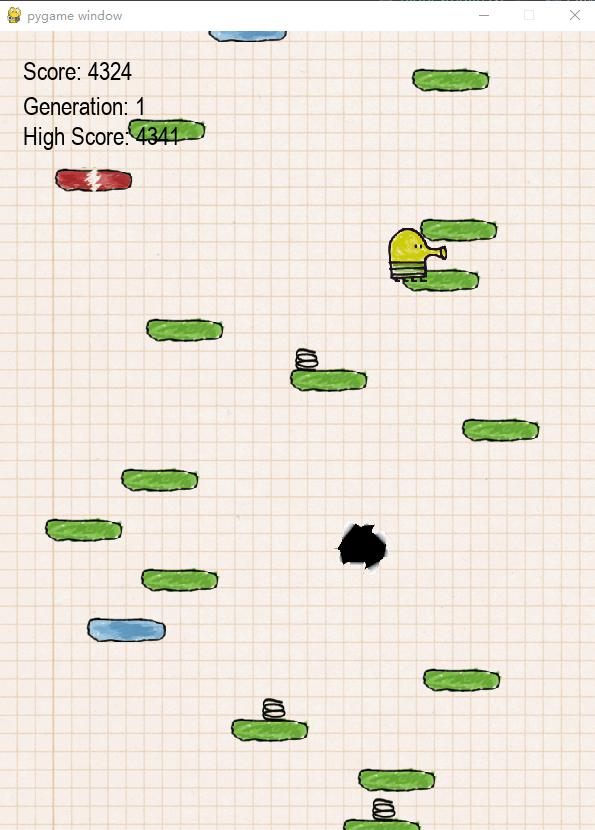
\includegraphics[width=0.42\textwidth]{1.png}
    \caption{The interface when the game is running. }
    \label{fig:game}
\end{figure}

%%%%%
\section{Genetic Algorithm AI}
\subsection{General GA}
   Genetic algorithm (GA) is a heuristic algorithm inspired by the process of natural selection that belongs to the larger class of evolutionary algorithms (EA). Genetic algorithms are commonly used to generate high-quality solutions to optimization and search problems by relying on biologically inspired operators such as mutation, crossover and selection. Some examples of GA applications include optimizing decision trees for better performance, solving sudoku puzzles, etc.
   In this game, we used a variant of genetic algorithm to train our AI.

\subsection{Advantages}
   The reason to use genetic algorithm is that it is hard for the neural network to update using back propagation with gradient decent. In this game, the only persuasive evaluation is the game score because it is hard to have an accurate evaluation of the current state the player is in. We can only calculate a score when a player dies or the game ends with exception. GA gives a convenient solution to the game: we can simply generate a dozen of players and make them compete. The one who lives till the end would have the highest score and will have a highest weight when generating the next generation, i.e. the next generation would be more similar to the player who owned the highest score. Though this would bring some local optimum problem, we can jump out of it by a greater randomness and a simple restart. GA is a quite effective algorithm for this problem.
   
\subsection{Implementation}
   Our implementation of GA is simple and crude. We hoped to extract useful features as network input. However, our game is not a offline policy based one but a real-time one, which means we need a small and simple network to guarantee the decision speed and interactivity. We used a simple fully-connected network.
\paragraph{Network}
   Network input is game state features, including platform x-coordinates, monster x-coordinates, blackhole x-coordinates, which were all relative positions to the player. The player also has perceptions of the surrounding objects, which includes platforms on different angles, monsters and springs. A fully-connected network is called a brain, and the structure is like below:\\

   $
   hidden=sigmoid(dot(input,weight1)+bias1)
   $

   $
   output=sigmoid(dot(hidden,weight2)+bias2)
   $\\
   
   The output contains the likelihood of two directions.The decision is made by choosing the bigger one. 
   
   As the most important part in our Genetic Algorithm, we apply genetic operators to our networks. To fit the features our game have, we chose mutate as a genetic method, but as we did not use crossover or regrouping methods, our GA is still a naive one. 

\paragraph{Process of game}
   When game starts, GA generates a generation of players with different brains, and the player will have a competition. The one who survives at last will be saved. After one generation, new players will be generated based on the brain of the last survivor. The weight of its brain is sampled using normal distribution of the original weights, and the variance can be reduced during game time. To avoid coincident death of players who have similar networks, we save some losers as well, and they also have weights in generating the next generation. To avoid the randomness of different maps, which results in different performance, the player with the highest score in history will be saved for the whole training, and it also have a weight in the next generations.
   
\begin{figure}[htbp]
    \centering
    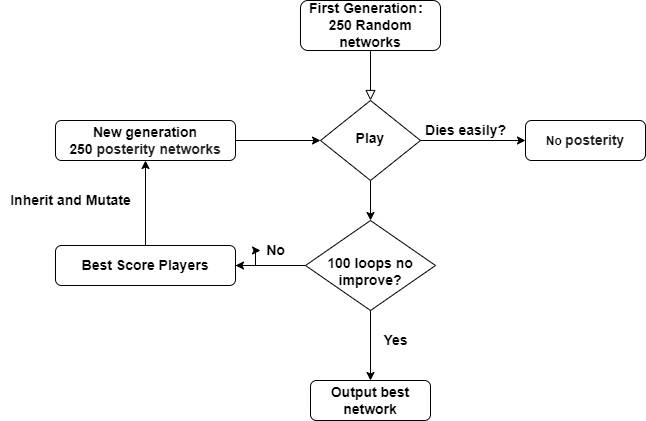
\includegraphics[width=0.48\textwidth]{2.png}
    \caption{Our logic of Genetic Algorithm training. }
    \label{fig:game}
\end{figure}

\subsection{Achievement or Result}
Our implementation is slightly different from the original game version. But we also made manual playing mode and tried our game by hand. Our AI can reach a high score of 100,000 while a human can only reach a score up to 20,000. However, a high score is hard to achieve because of the great randomness of our game, which means sometimes there may not be a solution that can do well. The player may be stuck in some situation. Though we tried to set random seeds to ensure that every time we generate the same map, it is hard to train an AI that fit all maps.

\subsection{Underlying Framework Limit}
\paragraph{Platform instability}
We failed to make sure that there exists a way to higher place all the time, which limits the learning result. 
\paragraph{Camera following}
Since the UI follows the highest player in the map, the players which jumped slow at the beginning will be left behind and be declared dead. That caused an “always left or always right” state in our early training, because GA is actually a competing algorithm and once a player can ensure to beat other players, i.e. make them die, it will be the winner. A player who goes always left or always right will interact with more platforms and have higher speed at the beginning of the game, and that’s enough for it to win most players. This is a defect of GA. Since it is hard to fit every player in a single map due to performance limit, this error can not be avoided, though it is not likely to happen.
\paragraph{Network size}
Our doodle jump game is a 60-tick real-time game, which means game state changes 60 times in a single second ideally. That means all calculations should end within $\frac{1}{60}$ second. So our network mustn't be too large, or we will lose the real-time reaction, have delay and trap in trouble. But small networks made us have short input length and can not describe the game world correctly and exhaustively. So the ignored details would hurt our player or limit it's decision.
%-------------------------------------------------------------------------
%%%
\section{Q-Learning AI}
Q-Learning is a traditional method for Reinforcement Learning. 
We have already implemented this method in the Pacman game introduced in our lecture.
Despite that the result is not good when facing several ghosts, the pacman can achieve a quite satisfying behaviour.
In the doodle jump game, we also tried to implement Q-Learning for decision-making, and achieved a quite good result.
In this project, the approximate Q-Learning method is used, taking reference of lecture project 5.
\subsection{State Representation}
The state representation in pacman searching problem is quite easy, when the state space is small enough to be stored.
However, in Doodle Jump, the state is very complicated as there are many platforms.
Therefore, only the approximate Q-Learning using features can be used.

The state mainly contains the player, the platforms that can be step on, and even the monsters and springs.
The actions are moving left, moving right and staying still. In each call of \verb|getQvalue()|, 
the player's position is predicted similarly used in moving part, as an expression of action.
The feature extractor used the predicted position to calculate the Q value of the current environment.
When the game updates, the real Q value is used to calculate the time difference and update the weights.
This is done in \verb|update()|.

\subsection{Feature Extraction}
In this part, some useful features are extracted for evaluating Q value of each state and action.

\subsubsection{Platforms}
   The platforms have different importance considering the different distance and height from the player.
   A general solution is to consider a platform that is above the player, which is most likely to be reached.
   This makes the player jumps slowly but safely.
   However, considering one platform is not enough, for that in some cases, the nearest above platform is away from the others.
   It is more likely for a human player to choose the direction that have more platforms, which is safer if he missed one step.
   Therefore, several platforms above are considered as features.

   To get a good result, the platform choice is complicated. Below is a some reference code. 
\begin{python}
# below is some codes of choosing part
# self is the player
   for p in platforms:
      ...
      # the below one is not too far
      if (abs(p.x - self.x) < 300):
         tmpCandidates.append(p.x)
      ...
      # check the p above is not too high
      if (self.startY + maxHeight < p.startY):
         break
      ...
      # check the p above is reachable
      isRight = (p.x - self.x) > 0
      farestDist = \
      self.jump*(self.xvel*2+self.jump*isRight) 
      if (abs(p.x - self.x) < abs(farestDist)):
         returnPlatforms.append(p.x + p.vel)
\end{python}
   To be noticed, only the platforms that are not too high, and are reachable after a whole jump, can be added into the feature.
   The \verb|tmpCandidates| stores the platforms below the player. When the player is falling, we don't want it to head for those above.
   On the contrary, it focuses on those below for landing. 
   These features are represented as possible platforms, which are the platforms the player intends to head to.

\subsubsection{Monsters}
   The monsters can also be used as features. However, because the monsters are not regularly placed than platforms, its weight is not very useful.
   In our test, there is not much difference when monster feature is added. 
   A probable reason is that because the weights are not updated simultaneously with platform weights when the monsters don't appear.
   So the old monster weight may not be influential when new platform weight are updated.

\subsubsection{Distance}
   The distance from player and platforms is directly related to the feature value.
   Intuitively, player will choose a near platform. He prefers a step right when a right platform is closer than a left one.
   Thus, when the distance change are the same, a nearer target platform needs a bigger Q-value difference to make the agent choose the action.
   Therefore, we took the log distance, in which $Q-value$ varies smaller when $distance$ are bigger.
   The agent will choose the nearer one when two platforms have the same weights.
\begin{python}
   feats['firstUpDist'] = math.log2(
      abs((upPlatforms[0] - player.x)/600)+1) 
\end{python}

\subsection{Results}
A demo training record is \href{qlearning.mp4}{here}.
Not like Generic Algorithm which uses neural network and update once each game.
The player agent updates its weight every game update.
So in the first game, the player can already achieve a quite good score.
To be observed, the score have a slight rise in the second and third game.
On average, the score can reach 25000+ after 3 or 4 games.

Actually, due to the simpleness of Q-Learning where the features have linear relation, 
the agent can hardly achieve as good result as using neural network.
We can observe that in several complex cases the agent may make a stupid decision.
However, as an AI it already achieves a good behavior.


\section{Conclusion}
We successfully transplanted the Doodle Jump game with a high degree of reduction. Then two AI training methods were used to successfully train the AI to play the game on its own. However, there are still some interesting open problems:
\begin{itemize}
    \item Many of the original game items have not been restored, such as rockets, protective shields.
    \item There is a large space for improvement in game mechanics, such as the problem of Platform instability.
    \item The results of the two or more AI training methods of this game can be quantitatively compared.
    \item Find a way to train the doodler to react better when he meets the monsters.
\end{itemize}








\end{document}
